\documentclass{article}
\usepackage[utf8]{inputenc}
\usepackage{hyperref}
\usepackage{color}
\usepackage[a4paper, total={6in, 8in}]{geometry}
\usepackage{subcaption}
\usepackage{amsmath}
\usepackage{natbib}
\setcitestyle{authoryear,open={(},close={)}} 
\usepackage{graphicx}
\usepackage{listings} 
\lstset{language=R,
    breaklines=true,
    basicstyle=\small\ttfamily,
    stringstyle=\color{DarkGreen},
    otherkeywords={0,1,2,3,4,5,6,7,8,9},
    morekeywords={TRUE,FALSE},
    deletekeywords={data,frame,length,as,character}
}
\usepackage{cleveref}
\usepackage{amsfonts}
\usepackage{authblk}
\usepackage{lineno} 
\usepackage[nomarkers,tablesonly,nofigures]{endfloat} %figure and table to the end
\linenumbers
\renewcommand{\baselinestretch}{2.0} 
 \renewcommand{\thefigure}{S\arabic{figure}}
 
  \title{Supplementary material of the manuscript:
 
 A comparison of spatial and non-spatial methods in statistical modelling of $NO_2$: prediction accuracy, uncertainty quantification, and model interpretation}
  \date{}  
  \author{}
\begin{document}

\maketitle
We calculated the Nash-Sutcliffe Model efficiency coefficient (NSE) of the XGBoost model in each spatial block after applying the random 10-fold Cross-Validation (CV) and compared it with the spatial-blocked CV. The spatial blocks of these two CV are defined the same way. Figure S1 shows the differences in the NSE between the 10-fold random CV and the spatial-blocked CV. More reddish colour indicates the spatial CV is being more pessimistic comparing to the 10-fold random CV and more greenish colour indicates the opposite. We could observe that leaving out the western Netherlands for testing in spatial CV may have caused extrapolating and therefore pessimistic accuracy assessment.  

\begin{figure}
    \centering
    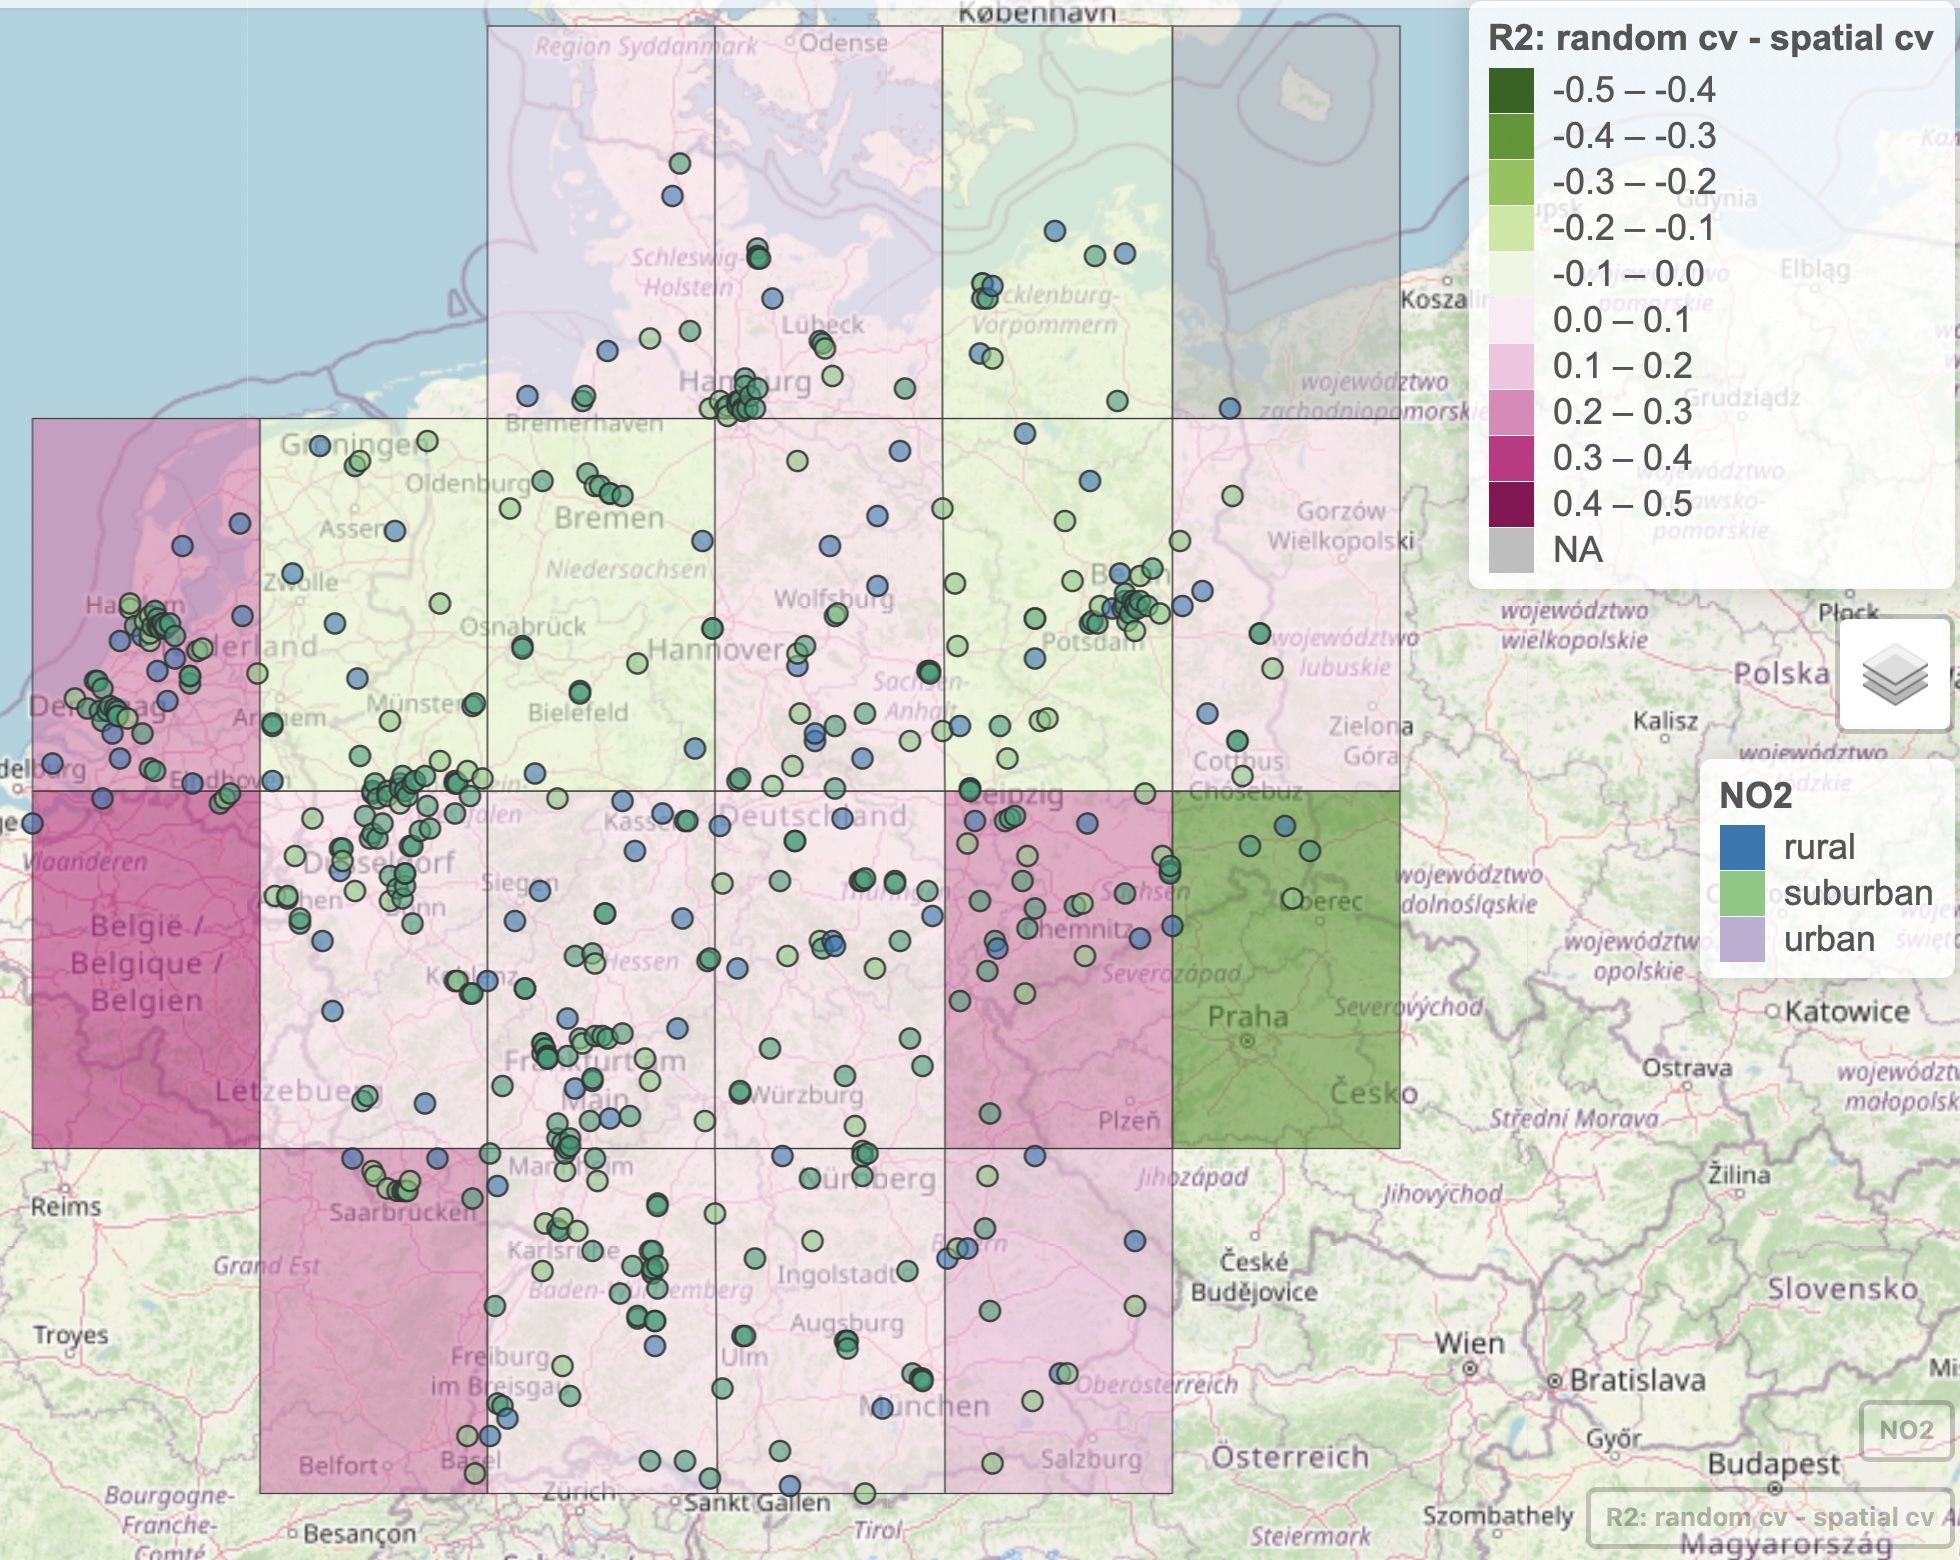
\includegraphics[scale=0.2]{s1.jpeg}
    \caption{Differences in the Nash-Sutcliffe Model efficiency coefficient for the XGBoost model between 10-fold random CV and spatial CV (i.e. subtracting the spatial CV from the 10-fold random CV). 
}
    \label{fig:histqq}
\end{figure}{}

\end{document}